\chapter{Diagramas de secuencia}

\section{Buscar, añadir y modificar elementos}

En este diagrama de secuencia se indica como funcionarían las funciones de buscar, añadir y modificar elementos de la bodega. 

\begin{figure}[h]
    \centering
    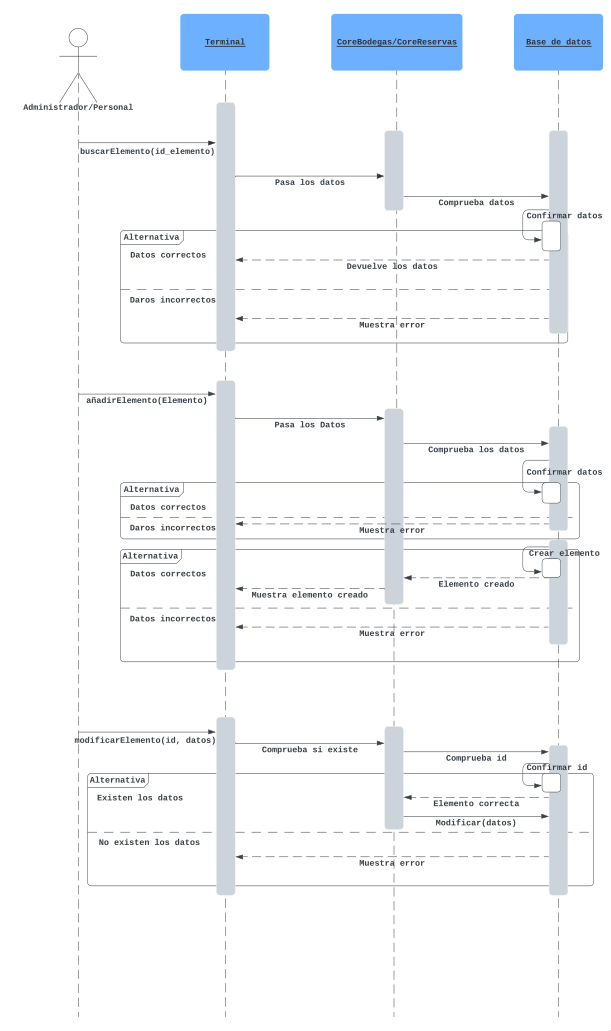
\includegraphics[width=0.4\textwidth]{figures/elementos-secuencia.png}
    \caption{Diagrama de secuencia de elementos}
    \label{fig:elementos}
\end{figure}

\section{Inicio de sesión}

En el segundo diagrama de secuencia veremos como funcionaría el programa de inicio de sesión.

\begin{figure}[h]
    \centering
    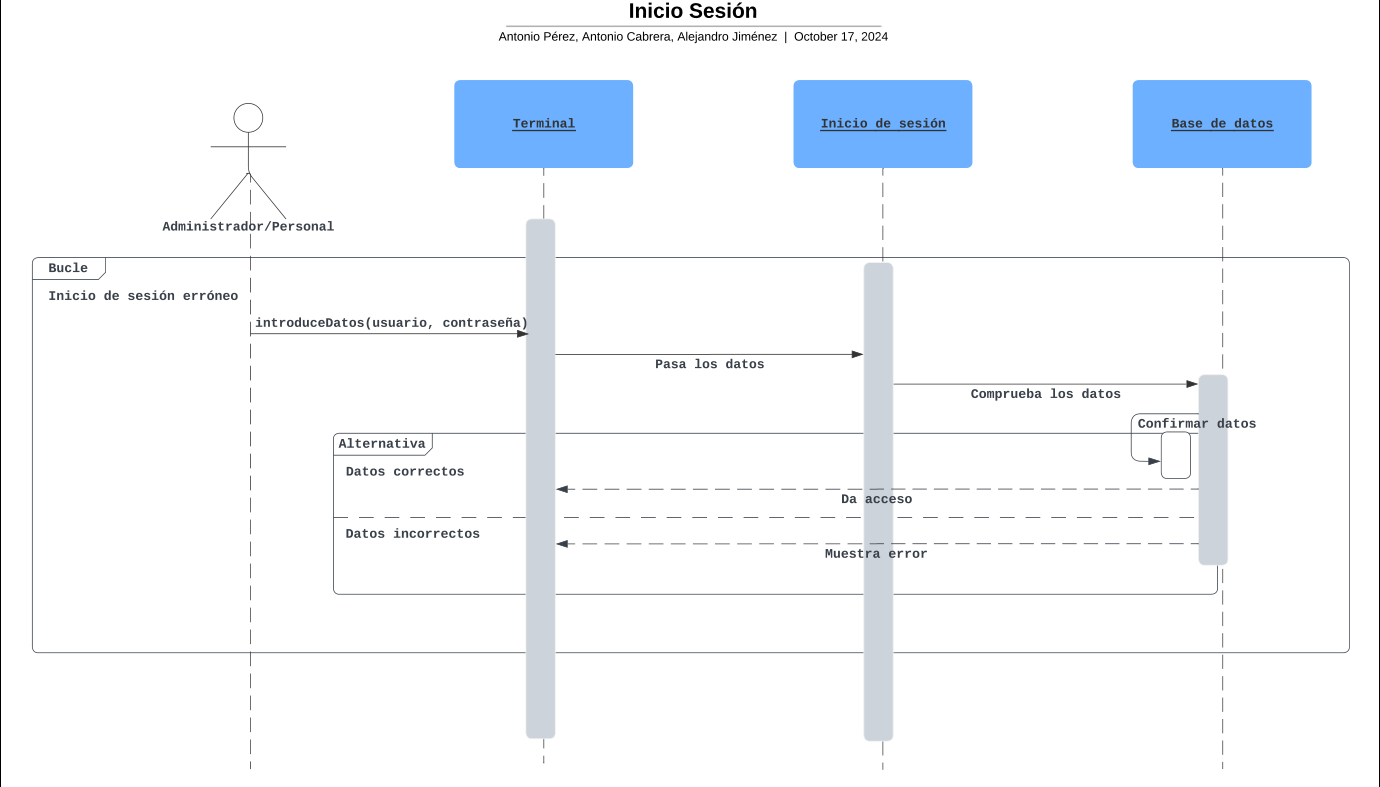
\includegraphics[width=1\textwidth]{figures/inicio-sesion-secuencia.png}
    \caption{Diagrama de secuencia de inicio de sesión}
    \label{fig:login}
\end{figure}

\pagebreak

\section{Personal secuencia}

Por último, en el siguiente diagrama se muestra el funcionamiento de las funciones que tienen que ver con la manipulación del personal.

\begin{figure}[h]
    \centering
    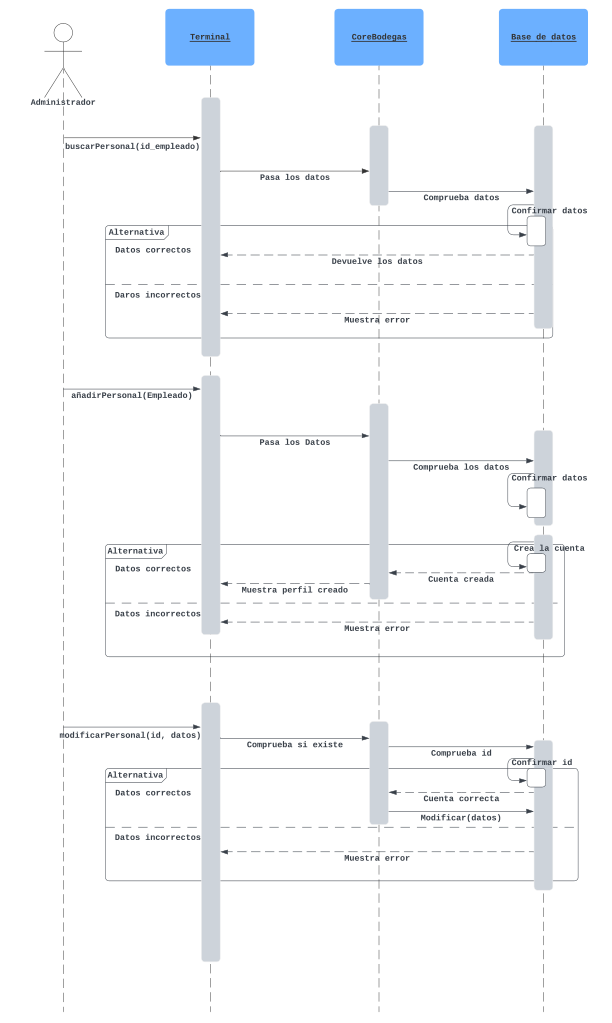
\includegraphics[width=0.5\textwidth]{figures/personal-secuencia.png}
    \caption{Diagrama de secuencia del personal}
    \label{fig:personal}
\end{figure}
